\chapter{Organization Essence Revealing}

The goals of this chapter are to perform an OER analysis as described in~\cite{dietz2015teoo,dietz2020enterprise}. For simplicity, we will only do the following steps: 

\begin{enumerate}
    \item Insert the project domain description into this document. 
    \item Perform the OER analysis and find \oact{ontological acts}. Be vigilant about the \btrap{blue traps}!
    \item Identify ontological transaction kinds and put them in the text. E.g. \oact{[TK1/rq]} If there are not enough red transactions, you can include the green ones. 
    \item Create an extended transaction result table (e-TRT). Map the transaction acts to the project domain description. See the~\cref{tab:etrt}. 
    \item Create a Subject-Actor table to realize the distinction between roles and DEMO actor roles. See the~\cref{tab:subjectactortable}. 
    \item Think in trees, not in flows and create the interaction structure of your transaction kinds. See the~\cref{fig:interactionStructure}.  
    \item Produce the Coordination Structure Diagram (CSD) and the Object Fact Diagram (OFD). See the~\cref{fig:csdModel} and ~\cref{fig:ofdModel}.  
    \item Finally, summarize your modeling thoughts and revelations. Don't forget about missing transaction steps table~\cref{tab:missing_transaction_steps}. 
\end{enumerate}

The process description of the Volley Case and it's OER analysis was taken from the Enterprise Ontology book~\cite{dietz2020enterprise}. 

%In the step 1 a coloring of the process description is made. The coloring can be done on text as well as on the flow chart diagram. 
\section{OER Step 1: Distinguishing Performa-Informa-Forma}

Legend: 
\begin{itemize}
    \item \oact{Ontological Act [Transaction Kind/Act type]}
    \item \btrap{Blue trap ontological act}!
\end{itemize}

\paragraph{\S 1 Preliminary Rules}

\begin{enumerate}[label={(\arabic*)}]
\item One can \oact{become member of the tennis club Volley[TK1]} by \btrap{sending a letter}\oact{[TK1/rq]} to the club by postal mail. In the letter one has to mention \iact{one’s surname and first name, birth date, gender, telephone number, and postal mail address (street, house number, zip code, and town)}. Adam, the administrator of Volley, \dact{empties the mailbox} daily and checks whether the information provided is complete. If not, he \dact{makes a telephone call} to the sender in order \iact{to complete the data}. Once a letter is complete, Adam \dact{writes an incoming mail number and the date on the letter, records the letter in the letter book, and puts it in a folder}. 
\item Every Wednesday evening, Adam \dact{takes the folder} to Eve, the secretary of Volley. He also \dact{takes the member register with him}. If Eve \oact{decides that an applicant can become member of Volley[TK1/pm]}, \dact{she stamps ‘new member’ on the letter and writes the date below it. She then hands the letter to Adam in order to add the new member to the member register. This is a book with numbered lines. Each new member is entered on a new line. The line number is the number by which the new member is referenced in the administration}. Next, Eve \iact{calculates the fee} that the new member \oact{has to pay [TK2]} for the remaining part of the calendar year. She asks Adam for the \iact{annual fee}, as \oact{decided at the general assembly [TK out of scope]}, which Adam \dact{has recorded on a sheet of paper}. Then, she asks Adam to \dact{write down the amount in the member register}. 
\item If Eve \oact{does not allow an applicant to become member[TK1/dc]} (e.g. because he or she is too young or because the maximum number of members has been reached), Adam will \btrap{send a letter}\oact{[TK2/rq]} in which he \iact{explains why the applicant cannot (yet) become member of Volley}.
\end{enumerate}

\paragraph{\S 2 Some Other Rules}

\begin{enumerate}[label={(\arabic*)}]
\item When all applications are processed, Adam \dact{takes the letters and the member register home} and \iact{prepares an invoice} to all new members for the \oact{payment of the first fee[TK2]}. He \btrap{sends these invoices}\oact{[TK2/rq]} \dact{by postal mail}. Payments have to be performed by bank transfers.
\item As soon as \btrap{a bank statement is received}\oact{[TK2/da]}, Adam \dact{prints a card} on which \iact{the member number, the starting date, the name, the date of birth, the gender, and the residence} are mentioned. \btrap{The card is sent}\oact{[TK1/da]} \dact{to the new member by postal mail}.
\end{enumerate}





\begin{landscape}
\section{OER Step 2: Identifying Transaction Kinds and Actor Roles}

\begin{table}[h]
\caption{Extended Transaction Result Table}
\label{tab:etrt}
\begin{tabular}{|l||l|l|}
\hline
Transaction  & Judgement by acknowledgement issuing (TK1) \\ \hline
Product      & Judgement by acknowledgement has been issued   \\ \hline
Initiator      & Defendant (CA1) \\ \hline
Executor       & Issuer of judgement by acknowledgement (AR1)      \\ \hline
Request        & Recognizes the claim (\S153a/1)   \\ \hline
Promise        & Not Specified   \\ \hline
Decline        &  Cannot be issued in matters in which a settlement cannot be concluded and approved  (\S153a/2)  \\ \hline
Declare        & Decide by a judgment according to that acknowledgement (\S153a/1)  \\ \hline
Reject         &  Not Specified   \\ \hline
Accept         & Not Specified (Probably Tacit) \\ \hline
Revoke Request & Not Specified \\ \hline
Revoke Promise & Not Specified \\ \hline
Revoke Declare & Not Specified  \\ \hline
Revoke Accept  &  Not Specified   \\ \hline
\end{tabular}
\end{table}

\begin{table}[h]
\caption{Extended Transaction Result Table}
\label{tab:etrt}
\begin{tabular}{|l||l|l|}
\hline
Transaction  & Issuing judgement in default (TK2) \\ \hline
Product  & Judgement in default has been issued \\ \hline
Initiator      &  Plaintiff (CA2)\\ \hline
Executor       &  Issuer of judgement in default (AR2)      \\ \hline
Request        & The plaintiff proposes it (\S153b/1)   \\ \hline
Promise        &  Not Specified (Probably Tacit)   \\ \hline
Decline        &  Cannot be issued in matters in which a settlement cannot be concluded and approved (\S153b/3) \\ \hline
Declare        & Decides on the action by judgment for default (\S153b/1) \\ \hline
Reject         &  Not Specified   \\ \hline
Accept         &  Not Specified (Probably Tacit) \\ \hline
Revoke Request &  Not Specified        \\ \hline
Revoke Promise &  Not Specified       \\ \hline
Revoke Declare &  Not Specified      \\ \hline
Revoke Accept  &  Not Specified             \\ \hline
\end{tabular}
\end{table}

\begin{table}[h]
\caption{Extended Transaction Result Table}
\label{tab:etrt}
\begin{tabular}{|l||l|l|}
\hline
Transaction  & Judgement in default declining (TK3)  \\ \hline
Product      & Judgement in default has been declined  \\ \hline
Initiator      &  Defendant (CA1)   \\ \hline
Executor       &  Judgement in default decline processor (AR3) \\ \hline
Request        & At the request of the defendant(\S153b/4)   \\ \hline
Promise        &  Not Specified \\ \hline
Decline        &  no later than the date on which the judgment becomes final (\S153b/4) \\ \hline
Declare        & Cancels the judgment and order a proceeding (\S153b/4) \\ \hline
Reject         &  Not Specified   \\ \hline
Accept         & Not Specified \\ \hline
Revoke Request & Not Specified  \\ \hline
Revoke Promise & Not Specified  \\ \hline
Revoke Declare & Not Specified  \\ \hline
Revoke Accept  &  Not Specified  \\ \hline
\end{tabular}
\end{table}

\begin{table}[h]
\caption{Extended Transaction Result Table}
\label{tab:etrt}
\begin{tabular}{|l||l|l|}
\hline
Transaction  &  Justification of the judgment correcting by court of first instance (TK4) \\ \hline
Product      & Justification of the judgement has been corrected \\ \hline
Initiator      &  Participant (CA3) \\ \hline
Executor       &  Correction of the justification first instance processor  (AR4)      \\ \hline
Request        &  Proposes correcting the justification (\S165/1)   \\ \hline
Promise        &  Not Specified  \\ \hline
Decline        &  The court does not comply (\S165/2)  \\ \hline
Declare        &  Decides on the correction (\S165/2) \\ \hline
Reject         &  Not Specified   \\ \hline
Accept         &  Not Specified (Probably Tacit) \\ \hline
Revoke Request &  Not Specified        \\ \hline
Revoke Promise & Not Specified     \\ \hline
Revoke Declare & Not Specified       \\ \hline
Revoke Accept  &  Not Specified     \\ \hline
\end{tabular}
\end{table}

\begin{table}[h]
\caption{Extended Transaction Result Table}
\label{tab:etrt}
\begin{tabular}{|l||l|l|}
\hline
Transaction  & Justification of the judgment correcting by court of second instance  (TK5) \\ \hline
Product      & Justification of the judgement has been corrected by court of appeal  \\ \hline
Initiator      &  Correction of the justification first instance processor (AR4) \\ \hline
Executor       &  Correction of the justification second instance processor (AR5) \\ \hline
Request        & Makes proposal to correct the reasoning of the judgment (\S165/2)  \\ \hline
Promise        &  Submits the case to the court of Appeal (\S165/2)    \\ \hline
Decline        &  Not Specified   \\ \hline
Declare        & Decides on the correction (\S165/2)  \\ \hline
Reject         &  Not Specified   \\ \hline
Accept         & Not Specified (Probably Tacit) \\ \hline
Revoke Request & Not Specified       \\ \hline
Revoke Promise & Not Specified  \\ \hline
Revoke Declare & Not Specified      \\ \hline
Revoke Accept  &  Not Specified \\ \hline
\end{tabular}
\end{table}

\begin{table}[h]
\caption{Extended Transaction Result Table}
\label{tab:etrt}
\begin{tabular}{|l||l|l|}
\hline
Transaction  &  Judgement completing (TK6) \\ \hline
Product      &  Judgement has been completed \\ \hline
Initiator      & Participant (CA3)  \\ \hline
Executor       &  Judgement completion performer (AR6) \\ \hline
Request        & Proposes that the judgment be completed (\S166/1)  \\ \hline
Promise        &  Not Specified    \\ \hline
Decline        &  The court rejects the proposal by resolution (\S166/2) \\ \hline
Declare        &  The completion shall be made by a court judgment (\S166/2)  \\ \hline
Reject         &  Not Specified   \\ \hline
Accept         & Not Specified (Probably Tacit) \\ \hline
Revoke Request & Not Specified       \\ \hline
Revoke Promise & Not Specified  \\ \hline
Revoke Declare & Not Specified      \\ \hline
Revoke Accept  &  Not Specified \\ \hline
\end{tabular}
\end{table}

\begin{table}[h]
\caption{Extended Transaction Result Table}
\label{tab:etrt}
\begin{tabular}{|l||l|l|}
\hline
Transaction  &  Resolution announcing (TK7) \\ \hline
Product      &   Resolution has been announced \\ \hline
Initiator      &  Resolution maker (AR7) \\ \hline
Executor       &  Resolution announcer (AR8) \\ \hline
Request        &  The court decides by a resolution(\S167/1)  \\ \hline
Promise        &  Not Specified   \\ \hline
Decline        &  Not Specified   \\ \hline
Declare        &  The resolution is announced to the present participants by the President of the Senate (\S168/2)  \\ \hline
Reject         &  Not Specified   \\ \hline
Accept         & Not Specified (Probably Tacit) \\ \hline
Revoke Request & Not Specified       \\ \hline
Revoke Promise & Not Specified  \\ \hline
Revoke Declare & Not Specified      \\ \hline
Revoke Accept  &  Not Specified \\ \hline
\end{tabular}
\end{table}

\begin{table}[h]
\caption{Extended Transaction Result Table}
\label{tab:etrt}
\begin{tabular}{|l||l|l|}
\hline
Transaction  &  Order for payment issuing (TK8) \\ \hline
Product      &  Order for payment has been issued \\ \hline
Initiator      &  Plaintiff (CA2) \\ \hline
Executor       &  Order for payment issuer (AR9) \\ \hline
Request        &   Not Specified (Probably Tacit)  \\ \hline
Promise        &    Not Specified   \\ \hline
Decline        &  Not Specified   \\ \hline
Declare        &  Issues order for payment(\S172/1)  \\ \hline
Reject         &  Not Specified   \\ \hline
Accept         & Not Specified (Probably Tacit) \\ \hline
Revoke Request & Not Specified       \\ \hline
Revoke Promise & Not Specified  \\ \hline
Revoke Declare & Not Specified      \\ \hline
Revoke Accept  &  Not Specified \\ \hline
\end{tabular}
\end{table}

\begin{table}[h]
\caption{Extended Transaction Result Table}
\label{tab:etrt}
\begin{tabular}{|l||l|l|}
\hline
Transaction  &  Paying the order for payment (TK9) \\ \hline
Product      &  The order for payment has been paid \\ \hline
Initiator      &  Order for payment issuer (AR9) \\ \hline
Executor       &  Order for payment payer (AR10) \\ \hline
Request        &    Court enforces payer to pay claims to plaintiff (\S172/1)
  \\ \hline
Promise        &    Not Specified   \\ \hline
Decline        &  Payer may fill an objection prior to the court (\S172/1)  \\ \hline
Declare        &  Issues order for payment(\S172/1)  \\ \hline
Reject         &  Not Specified   \\ \hline
Accept         & Not Specified (Probably Tacit) \\ \hline
Revoke Request & The court cancels order for payment (\S173/2)       \\ \hline
Revoke Promise & Not Specified  \\ \hline
Revoke Declare & Not Specified      \\ \hline
Revoke Accept  &  Not Specified \\ \hline
\end{tabular}
\end{table}

\begin{table}[h]
\caption{Extended Transaction Result Table}
\label{tab:etrt}
\begin{tabular}{|l||l|l|}
\hline
Transaction  &  Filing an appeal against an order for payment (TK10) \\ \hline
Product      &  The order for payment has been appealed \\ \hline
Initiator      &  Order for payment payer (AR10)  \\ \hline
Executor       &  Payment order appeal processor (AR11) \\ \hline
Request        & One of the defendants fills an appeal in time (\S174/2)
  \\ \hline
Promise        &    Not Specified   \\ \hline
Decline        & The court rejects the late appeal by resolution (174/3)  \\ \hline
Declare        &  Cancels the payment order in full and the court orders the hearing (\S174/2)  \\ \hline
Reject         &  Not Specified   \\ \hline
Accept         & Not Specified (Probably Tacit) \\ \hline
Revoke Request & Not Specified \\ \hline
Revoke Promise & Not Specified  \\ \hline
Revoke Declare & Not Specified      \\ \hline
Revoke Accept  &  Not Specified \\ \hline
\end{tabular}
\end{table}

\begin{table}[h]
\caption{Extended Transaction Result Table}
\label{tab:etrt}
\begin{tabular}{|l||l|l|}
\hline
Transaction  &  Electronic order for payment issuing (TK11) \\ \hline
Product      &  Electronic order for payment has been issued \\ \hline
Initiator      & Plaintiff (CA2) \\ \hline
Executor       &  Electronic payment order issuer (AR12) \\ \hline
Request        & Submitts a proposal by signing an electronic form (\S174a/1)
  \\ \hline
Promise        &    Not Specified   \\ \hline
Decline        & President of the Senate refuses proposal by resolution (174a/4)  \\ \hline
Declare        &  The court may issue an electronic payment order (\S174a/2)  \\ \hline
Reject         &  Not Specified   \\ \hline
Accept         & Not Specified (Probably Tacit) \\ \hline
Revoke Request & Not Specified \\ \hline
Revoke Promise & Not Specified  \\ \hline
Revoke Declare & Not Specified      \\ \hline
Revoke Accept  &  Not Specified \\ \hline
\end{tabular}
\end{table}

\begin{table}[h]
\caption{Extended Transaction Result Table}
\label{tab:etrt}
\begin{tabular}{|l||l|l|}
\hline
Transaction  &  Paying the electronic order of payment (TK12) \\ \hline
Product      &  Electronic order of payment has been paid \\ \hline
Initiator      &  Electronic payment order issuer (AR12) \\ \hline
Executor       &  Electronic payment order payer(AR13) \\ \hline
Request        &    Court enforces payer to pay claims to plaintiff (\S172/1)
  \\ \hline
Promise        &    Not Specified   \\ \hline
Decline        &  Payer may fill an objection prior to the court (\S172/1)  \\ \hline
Declare        &  Issues order for payment(\S172/1)  \\ \hline
Reject         &  Not Specified   \\ \hline
Accept         & Not Specified (Probably Tacit) \\ \hline
Revoke Request & The court cancels order for payment (\S173/2)       \\ \hline
Revoke Promise & Not Specified  \\ \hline
Revoke Declare & Not Specified      \\ \hline
Revoke Accept  &  Not Specified \\ \hline
\end{tabular}
\end{table}

\begin{table}[h]
\caption{Extended Transaction Result Table}
\label{tab:etrt}
\begin{tabular}{|l||l|l|}
\hline
Transaction  &  Filing an appeal against an electronic order for payment (TK13) \\ \hline
Product      &  The electronic order for payment has been appealed (TK13) \\ \hline
Initiator      &  Electronic payment order payer (AR13) \\ \hline
Executor       & Electronic Payment order appeal processor (AR14) \\ \hline
Request        & One of the defendants fills an appeal in time (\S174/2)
  \\ \hline
Promise        &    Not Specified   \\ \hline
Decline        & The court rejects the late appeal by resolution (174/3)  \\ \hline
Declare        &  Cancels the payment order in full and the court orders the hearing (\S174/2)  \\ \hline
Reject         &  Not Specified   \\ \hline
Accept         & Not Specified (Probably Tacit) \\ \hline
Revoke Request & Not Specified \\ \hline
Revoke Promise & Not Specified  \\ \hline
Revoke Declare & Not Specified      \\ \hline
Revoke Accept  &  Not Specified \\ \hline
\end{tabular}
\end{table}

\begin{table}[h]
\caption{Extended Transaction Result Table}
\label{tab:etrt}
\begin{tabular}{|l||l|l|}
\hline
Transaction  &  Issuing European order for payment (TK14) \\ \hline
Product      &  European order for payment has been issued \\ \hline
Initiator      &  Plaintiff (CA2) \\ \hline
Executor       & European payment order issuer (AR15) \\ \hline
Request        &    Obligee presents a bill of exchange or a check (\S175/1)
  \\ \hline
Promise        &    Not Specified   \\ \hline
Decline        &  Payer may fill an objection prior to the court (\S172/1)  \\ \hline
Declare        &  Issues order for payment(\S172/1)  \\ \hline
Reject         &  Not Specified   \\ \hline
Accept         & Not Specified (Probably Tacit) \\ \hline
Revoke Request & Not Specified    \\ \hline
Revoke Promise & Not Specified  \\ \hline
Revoke Declare & Not Specified      \\ \hline
Revoke Accept  &  Not Specified \\ \hline
\end{tabular}
\end{table}

\begin{table}[h]
\caption{Extended Transaction Result Table}
\label{tab:etrt}
\begin{tabular}{|l||l|l|}
\hline
Transaction  &  European payment order paying (TK15) \\ \hline
Product      &  European payment order has been paid \\ \hline
Initiator      &  European payment order issuer (AR15) \\ \hline
Executor       &  European payment order payer (AR16) \\ \hline
Request        &   The court orders the defendant to pay the required amount and costs within 15 days  (\S175/1)
  \\ \hline
Promise        &    Not Specified   \\ \hline
Decline        &  If the request for an order for payment cannot be granted, the court shall order a hearing.(\S175/1)  \\ \hline
Declare        &  Not Specified  \\ \hline
Reject         &  Not Specified   \\ \hline
Accept         & Not Specified (Probably Tacit) \\ \hline
Revoke Request & Not Specified      \\ \hline
Revoke Promise & Not Specified  \\ \hline
Revoke Declare & Not Specified      \\ \hline
Revoke Accept  &  Not Specified \\ \hline
\end{tabular}
\end{table}

\begin{table}[h]
\caption{Extended Transaction Result Table}
\label{tab:etrt}
\begin{tabular}{|l||l|l|}
\hline
Transaction  &   Appeal proceedings of European payment order opening (TK16) \\ \hline
Product      &  Appeal proceedings of European payment order has been opened \\ \hline
Initiator      &  European payment order payer (AR16)\\ \hline
Executor       &  European payment order appeal processor (AR17) \\ \hline
Request        &   Defendant fills an appeal in time (\S175/4) \\ \hline
Promise        &    Not Specified   \\ \hline
Decline        &  Late appeals or appeals which do not contain reasons shall be rejected by the court.(\S175/3)  \\ \hline
Declare        &  Not Specified  \\ \hline
Reject         &  Not Specified   \\ \hline
Accept         & Not Specified (Probably Tacit) \\ \hline
Revoke Request & If the defendant withdraws the appeal, the court shall suspend the appeal proceedings by a resolution (\S175/5)      \\ \hline
Revoke Promise & Not Specified  \\ \hline
Revoke Declare & Not Specified      \\ \hline
Revoke Accept  &  Not Specified \\ \hline
\end{tabular}
\end{table}


\begin{table}[h]
\caption{Subject Actor Table}
\label{tab:subjectactortable}
\begin{tabular}{|l|l|l|}
\hline
  & Issuer of judgement by acknowledgement (AR1)  &  Issuer of judgement in default (AR2)   \\ \hline
Defendant &  &  \\ \hline
Court & X & X  \\ \hline
Plaintiff &  &  \\ \hline
\end{tabular}
\end{table}

\begin{table}[h]
\caption{Subject Actor Table}
\label{tab:subjectactortable}
\begin{tabular}{|l|l|l|}
\hline
  & Judgement in default decline processor (AR3)  &  Correction of the justification first instance processor (AR4)   \\ \hline
Court &  & X  \\ \hline
\end{tabular}
\end{table}

\begin{table}[h]
\caption{Subject Actor Table}
\label{tab:subjectactortable}
\begin{tabular}{|l|l|l|}
\hline
  &  Correction of the justification second instance processor (AR5)  &  Judgement completion performer (AR6)   \\ \hline
Court & X & X  \\ \hline
\end{tabular}
\end{table}

\begin{table}[h]
\caption{Subject Actor Table}
\label{tab:subjectactortable}
\begin{tabular}{|l|l|l|}
\hline
  &  Resolution maker (AR7)  &  Resolution announcer (AR8)    \\ \hline
Defendant & X  &  \\ \hline
Court &  & X  \\ \hline
Plaintiff &  &  \\ \hline
\end{tabular}
\end{table}

\begin{table}[h]
\caption{Subject Actor Table}
\label{tab:subjectactortable}
\begin{tabular}{|l|l|l|l|}
\hline
  &  Order for payment issuer (AR9)  &  Order for payment payer (AR10) &  Payment order appeal processor (AR11)   \\ \hline
Defendant & X  &  \\ \hline
Court &  & X  \\ \hline
Plaintiff &  &  \\ \hline
\end{tabular}
\end{table}

\begin{table}[h]
\caption{Subject Actor Table}
\label{tab:subjectactortable}
\begin{tabular}{|l|l|l|}
\hline
    &  Electronic payment order issuer (AR12) &   Electronic payment order payer (AR13)   \\ \hline
Defendant & X  &  \\ \hline
Court &  & X  \\ \hline
Plaintiff &  &  \\ \hline
\end{tabular}
\end{table}

\begin{table}[h]
\caption{Subject Actor Table}
\label{tab:subjectactortable}
\begin{tabular}{|l|l|l|}
\hline
 &  Electronic payment order appeal processor (AR14)  &   European payment order issuer (AR15)   \\ \hline
Defendant & X  &  \\ \hline
Court &  & X  \\ \hline
Plaintiff &  &  \\ \hline
\end{tabular}
\end{table}

\begin{table}[h]
\caption{Subject Actor Table}
\label{tab:subjectactortable}
\begin{tabular}{|l|l|l|}
\hline
   &  European payment order payer (AR16) & European payment order appeal processor (AR17)    \\ \hline
Defendant & X  &  \\ \hline
Court &  & X  \\ \hline
Plaintiff &  &  \\ \hline
\end{tabular}
\end{table}

\end{landscape}

\section{OER Step 3: Composing the Essential Model}

Before starting with a CSD model, it is important to think about the transaction interaction structure. The transaction have to form one or more trees to compose into a process. You can see an example in~\cref{fig:interactionStructure}. 

\begin{figure}[h]\centering
	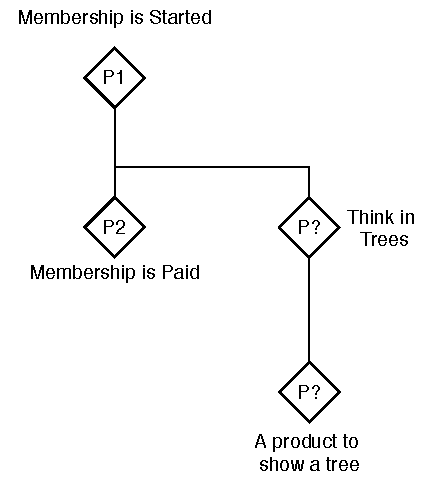
\includegraphics[width=8cm]{pic/VolleyInteractionStructure}
	\caption{An Interaction Structure Model of Volley}
	\label{fig:interactionStructure}
\end{figure}

\begin{figure}[h]\centering
	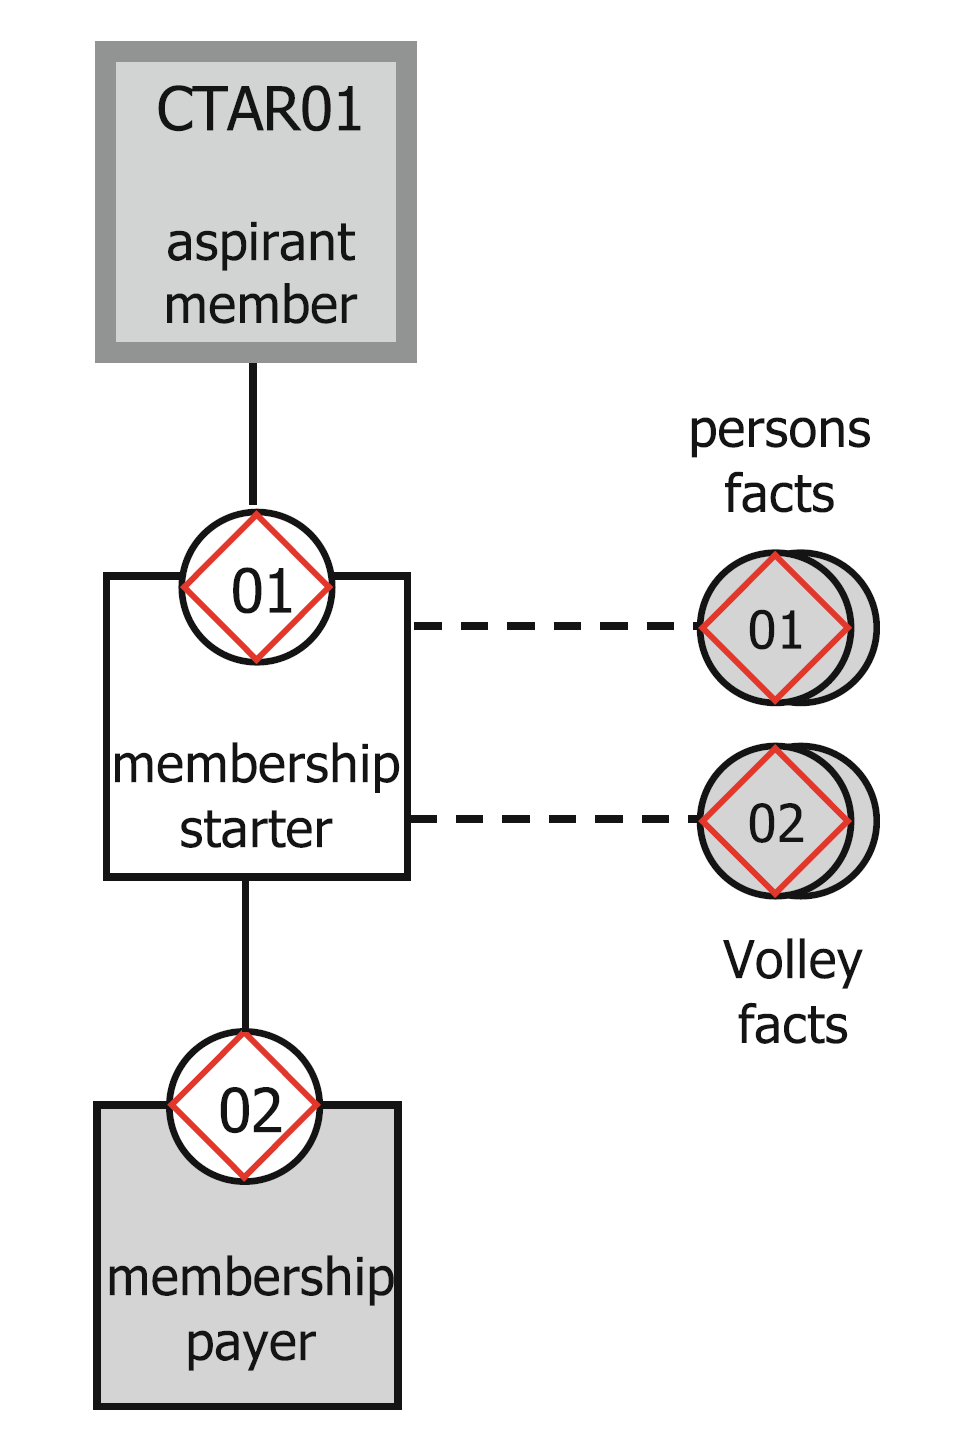
\includegraphics[width=6cm]{pic/VolleyCSD}
	\caption{A CSD Model of Volley~\cite{dietz2020enterprise}}
	\label{fig:csdModel}
\end{figure}

\begin{figure}[h]\centering
	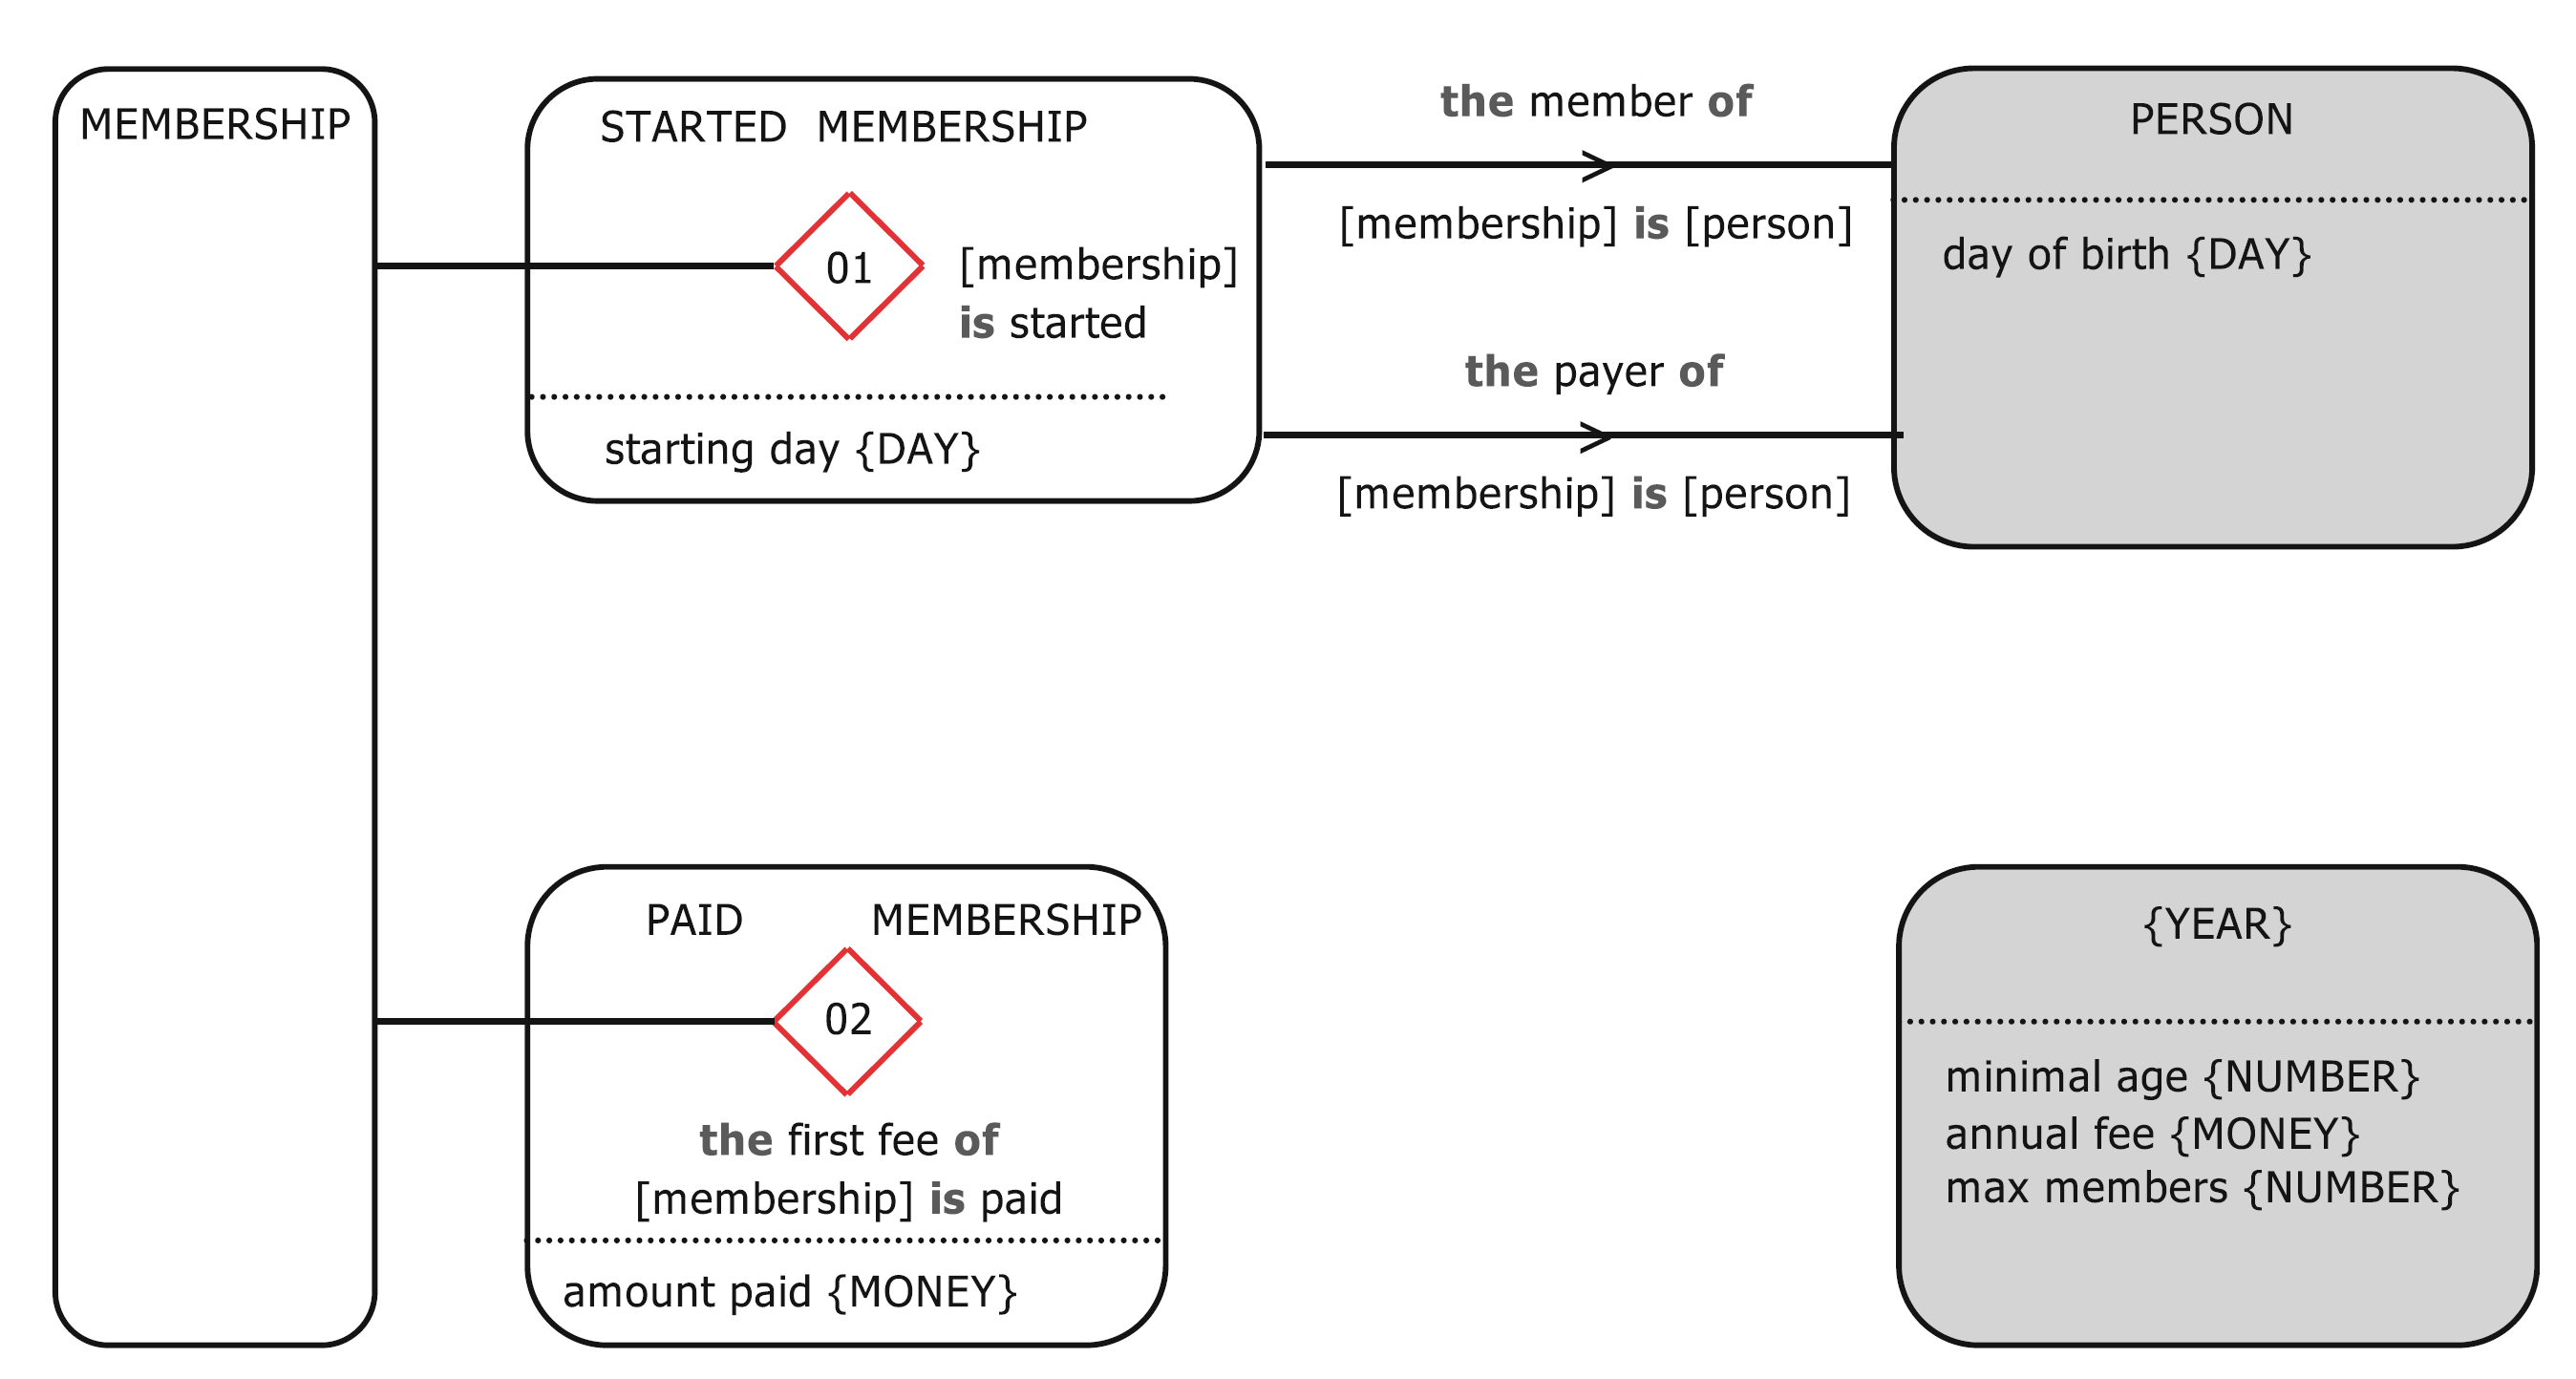
\includegraphics[width=12cm]{pic/VolleyOFD.png}
	\caption{An Object Fact Diagram of Volley~\cite{dietz2020enterprise}}
	\label{fig:ofdModel}
\end{figure}


\section{Summary}

Some comments about the OER analysis belong here. Why were you not able find some responsibilities? What was vaguely defined? Just roast the authors of the assignment (not the teachers :). 

And finally, show how much information is missing in a table~\cref{tab:missing_transaction_steps}. 

\begin{table}[h]\centering
\caption{Missing Transaction Steps}
\label{tab:missing_transaction_steps}
\begin{tabular}{|l||l|l|l|}
\hline
                      & Specified    & Not Specified & Missing Information \\ \hline
\multicolumn{4}{|c|}{Standard Transaction Pattern}                        \\ \hline
Request               & 2           & 0            & 0\%             \\ \hline
Promise               & 1           & 1            & 50\%            \\ \hline
Decline               & 1          & 1           & 50\%             \\ \hline
Declare               & 2           & 0            & 0\%              \\ \hline
Reject                & 0            & 2           & 100\%             \\ \hline
Accept                & 0           & 2            & 100\%            \\ \hline
\textbf{Total}        & \textbf{6} & \textbf{6}  & \textbf{50\%}   \\ \hline
\multicolumn{4}{|c|}{Revokes}                                             \\ \hline
Revoke Request        & 0            & 2           & 100\%             \\ \hline
Revoke Promise        & 0            & 2           & 100\%             \\ \hline
Revoke Declare        & 0            & 2           & 100\%            \\ \hline
Revoke Accept         & 0            & 2           & 100\%             \\ \hline
\textbf{Total}        & \textbf{0}   & \textbf{8} & \textbf{100\%}    \\ \hline
\multicolumn{4}{|c|}{Complete Transaction Pattern}                        \\ \hline
\textbf{Total}        & \textbf{6} & \textbf{14} & \textbf{70\%}    \\ \hline
\end{tabular}

\end{table}